\section{eo\-Value\-Param$<$ Value\-Type $>$ Class Template Reference}
\label{classeo_value_param}\index{eoValueParam@{eoValueParam}}
eo\-Value\-Param$<$Value\-Type$>$: templatized derivation of {\bf eo\-Param}{\rm (p.\,\pageref{classeo_param})}.  


{\tt \#include $<$eo\-Param.h$>$}

Inheritance diagram for eo\-Value\-Param$<$ Value\-Type $>$::\begin{figure}[H]
\begin{center}
\leavevmode
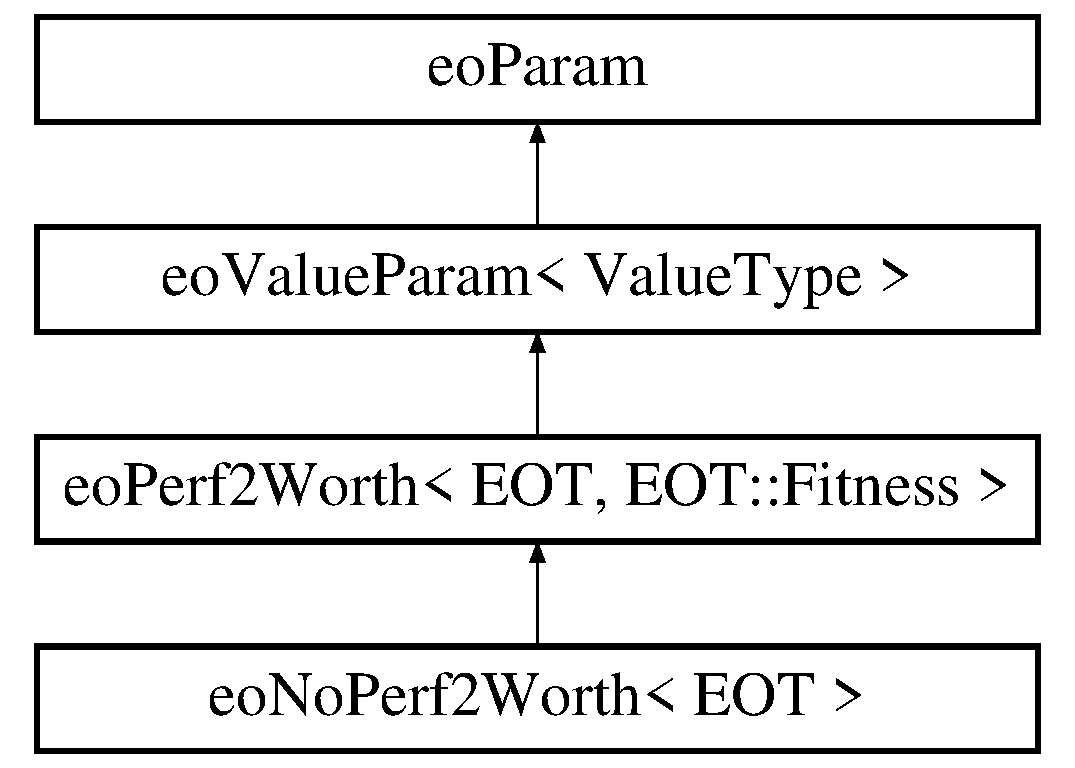
\includegraphics[height=4cm]{classeo_value_param}
\end{center}
\end{figure}
\subsection*{Public Member Functions}
\begin{CompactItemize}
\item 
{\bf eo\-Value\-Param} (void)\label{classeo_value_param_a0}

\begin{CompactList}\small\item\em Construct a Param. \item\end{CompactList}\item 
{\bf eo\-Value\-Param} (Value\-Type \_\-default\-Value, std::string \_\-long\-Name, std::string \_\-description=\char`\"{}No description\char`\"{}, char \_\-short\-Hand=0, bool \_\-required=false)
\begin{CompactList}\small\item\em Construct a Param. \item\end{CompactList}\item 
Value\-Type \& {\bf value} ()
\begin{CompactList}\small\item\em Parameter value. \item\end{CompactList}\item 
const Value\-Type \& {\bf value} () const 
\begin{CompactList}\small\item\em Parameter value. \item\end{CompactList}\item 
std::string {\bf get\-Value} (void) const \label{classeo_value_param_a4}

\begin{CompactList}\small\item\em Pure virtual function to get the value out. \item\end{CompactList}\item 
void {\bf set\-Value} (const std::string \&\_\-value)\label{classeo_value_param_a5}

\begin{CompactList}\small\item\em Pure virtual function to set the value. \item\end{CompactList}\end{CompactItemize}
\subsection*{Protected Attributes}
\begin{CompactItemize}
\item 
Value\-Type {\bf rep\-Value}\label{classeo_value_param_p0}

\end{CompactItemize}


\subsection{Detailed Description}
\subsubsection*{template$<$class Value\-Type$>$ class eo\-Value\-Param$<$ Value\-Type $>$}

eo\-Value\-Param$<$Value\-Type$>$: templatized derivation of {\bf eo\-Param}{\rm (p.\,\pageref{classeo_param})}. 

Can be used to contain any scalar value type. It makes use of std::strstream to get and set values. This should be changed to std::stringstream when that class is available in g++.

Note also that there is a template specialization for std::pair$<$double, double$>$ and for std::vector$<$double$>$. These stream their contents delimited with whitespace. 



Definition at line 136 of file eo\-Param.h.

\subsection{Constructor \& Destructor Documentation}
\index{eoValueParam@{eo\-Value\-Param}!eoValueParam@{eoValueParam}}
\index{eoValueParam@{eoValueParam}!eoValueParam@{eo\-Value\-Param}}
\subsubsection{\setlength{\rightskip}{0pt plus 5cm}template$<$class Value\-Type$>$ {\bf eo\-Value\-Param}$<$ Value\-Type $>$::{\bf eo\-Value\-Param} (Value\-Type {\em \_\-default\-Value}, std::string {\em \_\-long\-Name}, std::string {\em \_\-description} = {\tt \char`\"{}No\ description\char`\"{}}, char {\em \_\-short\-Hand} = {\tt 0}, bool {\em \_\-required} = {\tt false})\hspace{0.3cm}{\tt  [inline]}}\label{classeo_value_param_a1}


Construct a Param. 

\begin{Desc}
\item[Parameters:]
\begin{description}
\item[{\em \_\-default\-Value}]The default value \item[{\em \_\-long\-Name}]Long name of the argument \item[{\em \_\-description}]Description of the parameter. What is useful for. \item[{\em \_\-short\-Name}]Short name of the argument (Optional) \item[{\em \_\-required}]If it is a necessary parameter or not \end{description}
\end{Desc}


Definition at line 151 of file eo\-Param.h.

\subsection{Member Function Documentation}
\index{eoValueParam@{eo\-Value\-Param}!value@{value}}
\index{value@{value}!eoValueParam@{eo\-Value\-Param}}
\subsubsection{\setlength{\rightskip}{0pt plus 5cm}template$<$class Value\-Type$>$ Value\-Type\& {\bf eo\-Value\-Param}$<$ Value\-Type $>$::value ()\hspace{0.3cm}{\tt  [inline]}}\label{classeo_value_param_a2}


Parameter value. 

\begin{Desc}
\item[Returns:]parameter value \end{Desc}


Definition at line 166 of file eo\-Param.h.

Referenced by eo\-No\-Perf2Worth$<$ EOT $>$::operator()(), eo\-File\-Snapshot::operator()(), eo\-FDCStat$<$ EOT $>$::operator()(), and eo\-Parser::set\-Stop\-On\-Unknown\-Param().\index{eoValueParam@{eo\-Value\-Param}!value@{value}}
\index{value@{value}!eoValueParam@{eo\-Value\-Param}}
\subsubsection{\setlength{\rightskip}{0pt plus 5cm}template$<$class Value\-Type$>$ const Value\-Type\& {\bf eo\-Value\-Param}$<$ Value\-Type $>$::value () const\hspace{0.3cm}{\tt  [inline]}}\label{classeo_value_param_a3}


Parameter value. 

This is an overloaded member function, provided for convenience. It differs from the above function only in what argument(s) it accepts.

\begin{Desc}
\item[Returns:]parameter value \end{Desc}


Definition at line 175 of file eo\-Param.h.

The documentation for this class was generated from the following file:\begin{CompactItemize}
\item 
eo\-Param.h\end{CompactItemize}
